\documentclass[12pt]{article}
\usepackage[margin=1.2in]{geometry}
\usepackage[all]{nowidow}
\usepackage[hyperfigures=true, hidelinks, pdfhighlight=/N]{hyperref}
\usepackage[separate-uncertainty=true,group-digits=false]{siunitx}
\usepackage{graphicx,amsmath,physics,tabto,float,amssymb,pgfplots,verbatim,tcolorbox}
\usepackage{listings,xcolor,subfig,keyval2e,caption,import}
\numberwithin{equation}{section}
\numberwithin{figure}{section}
\definecolor{stringcolor}{HTML}{C792EA}
\definecolor{codeblue}{HTML}{2162DB}
\definecolor{commentcolor}{HTML}{4A6E46}
\lstdefinestyle{appendix}{
    basicstyle=\ttfamily\footnotesize,commentstyle=\color{commentcolor},keywordstyle=\color{codeblue},
    stringstyle=\color{stringcolor},showstringspaces=false,numbers=left,upquote=true,captionpos=t,
    abovecaptionskip=12pt,belowcaptionskip=12pt,language=Python,breaklines=true,frame=single}
\lstdefinestyle{inline}{
    basicstyle=\ttfamily\footnotesize,commentstyle=\color{commentcolor},keywordstyle=\color{codeblue},
    stringstyle=\color{stringcolor},showstringspaces=false,numbers=left,upquote=true,frame=tb,
    captionpos=b,language=Python}
\renewcommand{\lstlistingname}{Appendix}
\pgfplotsset{compat=1.17}

\title{The Magnetic Field of a Circular Coil: Induction and Inductance}
\author{KDSMIL001 \; PHY2004}
\date{\textbf{2 October 2020}}

\begin{document}
    \begin{titlepage}
        \maketitle
        \center
        \tableofcontents
    \end{titlepage}
    
    \section{Introduction and Aim}
    In this practical we investigated the behaviour of the magnetic field produced due 
    to an alternating current in a circular coil. This was done primarily by examining 
    the induced voltage in a search coil placed near the primary coil. 

    \section{Apparatus}
    The following equipment was used:
    \begin{itemize}
        \item Signal generator
        \item Power amplifier
        \item Ammeter
        \item Primary coil with 120 winds and diameter $\SI{6.8\pm0.1e-2}{\metre}$
        \item Secondary "search" coil with 175 winds and diameter $\SI{1.3\pm0.1e-2}{\metre}$
        \item Oscilloscope
    \end{itemize}
    The current in the primary coil was supplied by the amplifier, which was driven with a
    2 $V_{pp}$ sinusoidal signal from the signal generator. The ammeter was connected in 
    series with the coil in order to monitor the current in the circuit. This ammeter 
    displayed in rms, not amplitude, so we multiply by $\sqrt 2$ in order to get the 
    amplitude. Below is the set-up of the circuit.
    \begin{figure}[H]
        \begin{center}
           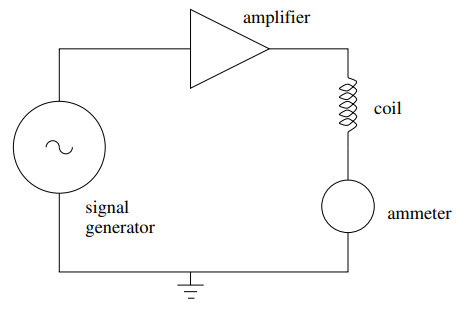
\includegraphics[width=.65\textwidth]{PrimaryCircuit.png}
           \caption{The primary circuit}
           \label{fig:PrimaryCircuitDiagram}
        \end{center}
    \end{figure}
    Additionally, we had our secondary coil connected to an oscilloscope in order to monitor 
    the induced emf $\epsilon$. This search coil was placed on a contraption that allowed us 
    to hold it at set distances from the primary coil, along the primary coil's axis. 

    \section{Experiment}
    \subsection{Field on the axis of a circular coil}
    In this section we looked specifically at the relationship between magnetic field 
    $\vec{B}(\vec{r},t)$ and induced $\epsilon$. First we look at Faraday's law, which says 
    \begin{equation}
        \epsilon=-N_1\frac{d}{dt}\int\vec{B}\cdot d\vec{A}
        \label{eqn:Faradays Law}
    \end{equation}
    In our case, we are aligning things in a way to have the magnetic field dependent only on 
    the distance $z$ from the primary coil. We also say that the magnetic field is directed 
    along the $z$-axis, approximately, allowing us to consider amplitudes only. So we have 
    \begin{align*}
        B(z,t)&\approx B(z)\cos(\omega t)\\
        \implies \epsilon&\approx -N_a A \frac{d}{dt}(B(z)\cos(\omega t))\\
        &=N_a AB(z)\omega\sin(\omega t)\\
        \implies B(z)&\approx \frac{\epsilon}{N_a A \omega}
    \end{align*}
    where $N_a$ is the number of winds in the search coil (175), $A$ is the cross-sectional 
    area of the search coil, $\omega$ is the angular frequency that the primary coil is being 
    driven at ($2\pi f$), and we have taken $\sin(\omega t)$ to be 1 as we are only interested 
    in amplitudes. We now have a kind of ``calibration factor", so when we measure the emf 
    induced in the search coil, we can immediately know the approximate value of the magnetic 
    field that induced it, i.e. the magnetic field produced by the primary coil. \newline
    We have a way of determining the magnetic field from the induced voltage, but we also want 
    to know how well that method agrees with what we would expect from the primary coil. The 
    magnitude of the magnetic field on the axis of a circular coil of radius $a$ is
    \begin{equation}
        B(z,t)=\frac{\mu_0 N I(t)}{2}\frac{a^2}{(a^2+z^2)^\frac{3}{2}}
        \label{eqn:MagFieldOnAxis}
    \end{equation}
    where $\mu_0=\num{4\pi e-7}$ is the permeability of free space, $N$ is the number of winds
    on the coil (120), and $I(t)=I_0\cos(\omega t)$. Again we can take the $\cos$ term to 
    be 1 as we're looking at amplitudes, which leaves us with 
    \begin{equation*}
        B(z)=\frac{\mu_0 N I_0}{2}\frac{a^2}{(a^2+z^2)^\frac{3}{2}}
    \end{equation*}
    Finally we collected some data: \newline
    We ran the signal generator at 
    $\SI{1000}{\hertz}=\SI{2000\pi}{\radian\second^{-1}}$ and $2V_{pp}$, with the amplifier 
    setting the current to $I_{rms}=\SI{0.353\pm0.00289}{\ampere}=\SI{0.49498\pm0.00409}{\ampere}$. 
    This uncertainty comes from reading the current off of our ammeter, which displayed 
    $\SI{0.35}{\ampere}$ rms, so we use a digital pdf with uncertainty $\frac{a}{2\sqrt3}$ 
    and $a=0.01$ to find $u(I_{rms})=0.00289$, so $u(I_0)=0.00289\sqrt{2}=0.00409$. \newline
    The cross-sectional area of the search coil is $A=(\num{6.5e-3})^2\pi=\SI{1.3273\pm0.0204e-4}{\metre^2}$. 
    This uncertainty comes from the uncertainty on the measurement of the diameter of the 
    search coil, using the formula $u(x^n)=|n|x^{n-1}u(x)$. \newline
    The uncertainty on any experimentally determined $B$ comes from the equation 
    \begin{equation*}
        u(B)=u(\frac{\epsilon}{N_a A\omega})=\frac{\epsilon}{N_a A\omega}\sqrt{\left( \frac{u(\epsilon)}{\epsilon}\right)^2+\left( \frac{u(A)}{A}\right)^2+\left( \frac{u(\omega)}{\omega}\right)^2}
    \end{equation*}
    where $u(\omega)$ is 2\% of the scale used on the display of the signal generator, which 
    was $1 kHz$, so $u(\omega)=0.02\cdot2000\pi=40\pi$, and $u(\epsilon)$ is determined from 
    the 2\% uncertainty of the display of the oscilloscope combined with the digital measurement 
    uncertainty
    \begin{align*}
        u(\epsilon)&=\sqrt{0.02^2+\left(\frac{\num{1e-5}}{2\sqrt3}\right)}\\
        &=0.01
    \end{align*}
    Below is the data and the theoretical model
    \begin{figure}[H]
        \begin{center}
           \scalebox{.7}{\subimport*{Data}{FieldAxisData.pgf}}
           \caption{Magnetic field determined using the calibration factor and $\epsilon$ 
           induced in a search coil due to a large primary coil, along with the theoretical 
           prediction made using \autoref{eqn:MagFieldOnAxis}}
           \label{fig:FieldAxisData}
        \end{center}
    \end{figure}
    
    \subsection{Induction}
    This section focuses on the effect of a varying frequency of alternating current on the 
    system we're investigating. For simplicity's sake we moved the coil to position $z=0$ and 
    varied the resistance from 100 Hz to 2 kHz. We didn't operate below 100 Hz as that would 
    result in an increase in 

\end{document}